\chapter{Usability Test}\label{ch:outlook}

Aufbauend auf allen bisher getätigten Analysen und Anpassungen des Interfaces, gilt es abschließend noch den Prototypen und die Implementierung mithilfe eines Usability Tests zu evaluieren.
Hierbei wird im Schritt "Finalize the UX design" des Human-centered design process die Rolle des Usability Testers abgedeckt, auf weitere Anpassungen in der Funktion des User Interface Designers wird verzichtet.

In diesem abschließenden Kapitel werden die Grundlagen des verwendeten Tools für den Usability Test erläutert.
Darauf folgend wird die Art des durchgeführten Tests erläutert und dargelegt auf welchen Grundlagen diese Wahl getätigt wurde.
Aufbauend auf den theoretischen Erläuterung wird die letzendliche Testaufgabe konkret definiert und die nötigen Anweisungen, sowie die Materialien zur Auswertung der Tests erstellt.
Abschließend werden die Ergebnisse der durchgeführten Auswertungen der Tests dargestellt und interpretiert, bevor noch ein Vergleich zwischen der bestehenden Software und den Verbesserungen gezogen wird.

\section{Lookback}

Bei Lookback handelt es sich um eine Cloudbasierte Softwarelösung, die es ermöglicht User Experience geräteübergreifend zu dokumentieren.
Bei der Durchführung der Tests besteht die Möglichkeit als Tester aktiv am Test teilzunehmen, oder die Probanden unmoderiert mit dem Prototyp oder der Software interagieren zu lassen.
Möchte der Usability Tester aktiv am Test teilnehmen kann hier auch noch aus den zwei Möglichkeiten gewählt werden, sich mit dem Nutzer innerhalb einer Live-Session oder  auch persönlich vor Ort an einem Rechner zu treffen.

Für die durchzuführenden Tests erstellt der Usability Tester innerhalb Loobacks ein Projekt.
Zugunsten des Datenschutzes besteht hier die Möglichkeit die Projekte auf privat zu setzen und nur ausgewählten Personen des Teams Zugriff zu den Aufnahmen zu gewähren.
Innerhalb des Projekteinstellungen können Instruktionen für die Nutzer bereit gestellt werden, die während des Test erscheinen und ihn durch die Aufgaben führen.
Das ist vor allem für den Fall hilfreich, wenn die Testperson den Test alleine durchführen soll.

Sollte der Test nicht persönlich stattfinden kann mithilfe eines Links kann der Test mit den Probanden geteilt werden, und der Tester bekommt eine Benachrichtigung sobald der Proband den Test alleine durchführt oder er dazustoßen kann.
Während der Session hat der Tester die Möglichkeit mit Zeitstempel versehene Notizen zu machen oder mit eventuell teilnehmen Teamkollegen zu chatten.
Diese Möglichkeit der Live\-Dokumentation erleichtert die folgende Auswertung des Test ungemein, da man sofort Auffälligkeiten festhalten kann und diese in der Aufzeichnung dadurch leichter auffindbar sind.
Nach Abschluss des Tests speichert Looback die Aufnahme in der Cloud, wodurch diese für die nachträgliche Auswertung des Tests abrufbar bleibt. \cite{.10.01.2020}

Die Möglichkeit der Live\-Dokumentation bildet das ausschlaggebende Argument für die Wahl des Tools, ebenfalls besteht die Möglichkeit in der hochgeladenen Aufnahme Kommentare hinzuzufügen, was die Auswertung sehr erleichtert.
Zusätzlich ist es wichtig den Test online durchführen zu können, da viele Modellierer nicht am Hauptstandort von EB beschäftigt sind, wodurch persönliches Testen nicht immer möglich ist.

\section{ Remote Usability Test}

%\paragraph{Deduktive und Induktive Tests}
%Usability Tests lassen sich grundsätzlich in deduktive und induktive Tests unterteilen.
%Letztere dienen hierbei der formativen Evaluation und werden genutzt um Prototypen oder Vorabversionen einer Software zu analysieren.
%Mithilfe dieser Analysen sollen vorhandene Schwachstellen aufgedeckt und Ideen für Verbesserungen gewonnen werden.
%Üblicherweise wird bei induktiven Tests nur ein System oder Prototyp getestet.

%Im Gegensatz dazu werden bei deduktiven Tests immer mehrere Alternativen einer Software miteinander verglichen, um mithilfe einer summativen Evaluation die einzelnen Systeme in ihrer Leistungsfähigkeit beurteilen zu können.
%Ebenfalls können mit dieser Art von Test gewünschte Verbesserungen in der Entwicklung eines Systems überprüft werden.
%Wie bei den formativen Tests ist es hier ebenfalls möglich Gestaltungs- und Verbesserungsvorschläge zu erhalten.\cite{Sarodnick.2016}
%Da in dieser Arbeit eine bestehende und überarbeitete Software Version verglichen werden liegt hier ein deduktiver Test vor.

%\paragraph{Remote und In Person Tests}
In Person Tests finden in der Regel in einem Usability Labor statt.
Dies bezeichnet einen abgeschlossener Raum ohne Störungsquelle, der mit aller benötigte Hard- und Software ausgestattet ist und in dem sich nur der Proband und der durchführende Tester aufhalten.

Bei einem Remote Usability Test wird die Arbeitsaufgabe nicht gemeinsam im Labor, sondern räumlich getrennt durchgeführt.
Hier lässt sich noch zwischen in Asynchronen und Synchronen Tests unterscheiden.
Bei letzteren besteht, trotz der räumlichen Trennung, eine direkte Verbindung mithilfe von Webcam und Sprachanruf, zwischen Tester und Proband.
Gleichzeitig dazu wird der Bildschirminhalt der Testperson übertragen, um es dem Tester zu ermöglichen dessen Interaktionen  zu verfolgen und durch den Test führen zu können.
Durch diese direkte Verbindung ist es ebenfalls möglich während, oder unmittelbar nach dem Test Fragen zu stellen.
Bei synchronen Tests besteht der Vorteil darin, mit geringem Aufwand sehr weit verteilte Nutzergruppen in den Test einbinden zu können.
Zusätzlich dazu findet der Test in der gewohnten Umgebung des Nutzers statt, es wird also keine ungewohnte Situation in einem Labor geschaffen, was die Nervosität der Nutzer eventuell steigern könnte.
Auch können die Probanden hier mit ihrer gewohnten Hard- und Software arbeiten, was vor allem für repräsentative Werte die die Effizienz betreffen von Vorteil ist.
Durch den Umstand der gewohnten Arbeitsumgebung entsteht jedoch in vielen Fällen auch ein technische Zusatzaufwand auf Seiten des Nutzers.
So kann es beispielsweise nötig werden sich Headset und Webcam anzuschaffen, oder zusätzliche Software auf dem Arbeitsgerät installieren zu müssen.
Dies tritt in einem Usability Labor nie auf, da hier eine einmalige Einrichtung der benötigten Hard- und Software stattfindet die exakt au den geplanten Test ausgelegt ist.

Im Rahmen eines asynchronen Tests besteht zusätzlich zu der räumlichen, auch noch eine zeitliche Trennung von Proband und Tester.
Identisch zum synchronen Test werden hier Gesicht und Bildschirminhalt der Testperson aufgezeichnet, der Nutzer kann jedoch aufgrund der Unabhängigkeit den Test zu einer ihm passenden Zeit durchführen.
Da er dadurch jedoch auch auf sich allein gestellt ist, empfiehlt es sich zusätzliche Kommentare und Fragebögen in den Test einzubauen um die direkte Befragung und Hilfestellung des synchronen Tests zu ersetzen.
Wie bei der synchronen Variante betseht hier der Vorteil das mit geringem Aufwand großräumig verteilte Nutzergruppen eingebunden werden können.
Zusätzlich können durch die vollautomatische Erfassung in dieser Variante auch sehr große Nutzergruppen effizient evaluiert werden.
Allerdings einstehen durch die zeitliche Trennung die NAchteile, das abgesehen von der Aufnahme keine Beobachtungsdaten existieren.
Es kann also beispielsweise nicht darum gebeten werden etwas genauer zu erläutern oder einen anderen Lösungsweg zu versuchen.
Die wohl größte Problematik bildet jedoch die Tatsache, dass nicht auf unerwartete Handlungen des Nutzers reagiert werden kann, was vor allem bei nur teilweise funktionalen Prototypen fatal sein kann.
Versuchen die Probanden hier einen Lösungsweg einzuschlagen, der in der vorliegenden Softwareversion nicht implementiert ist und auch nicht bedachte wurde, bekommt die Testperson eventuell auf keine Art und Weise eine Rückmeldung des Systems.
Diese Tatsache kann ohne weitere Unterstützung durch den Tester eventuell zum Abbruch des Test führen, was zu Unzufriedenheit auf Seiten des Testers und Nutzers führt.\cite{Sarodnick.2016}

Da Lookback jeden der eben erläuterten Tests unterstützt, wirkt sich das Tool auch nicht einschränkend aus und die Wahl kann aufgrund tatsächlich relevanter Tatsachen getroffen werden.
Aufgrund der Tatsache das innerhalb der Testaufgabe mit einem Prototyp interagiert werden muss, ist ein synchroner Test dem asynchronen vorzuziehen.
Da nicht alle in Guide zur Verfügung stehenden Interaktionsmöglichkeiten simuliert, und die Funktion \glqq publish to template interface\grqq{} verlagert wurde ist es wahrscheinlich, dass die Probanden an gewissen Punkten Unterstützung benötigen.
Es ist auch zu erwarten das bei den neuen Funktionen Fragen bei den Testpersonen auftauchen werden, die nicht alle in der Arbeitsaufgabe beantwortet werden können.
Im Gegensatz dazu wird auch Tester einige Aktionen genauer hinterfragen wollen oder herausfinden wollen warum gewisse Aktionen nicht durchgeführt wurden.

Grundlegend ist ein Test im Usability Labor, aufgrund der Ungestörtheit, immer dem Remote Test vorzuziehen.
Zum einen erstreckt sich die Nutzergruppe für diese Arbeit  jedoch über mehrere Firmenstandorte von Elektrobit, weshalb es nicht möglich ist den Test mit allen Probanden in einem Labor durchzuführen.
Zum anderen soll mithilfe Tests überprüft werden ob eine Effizienzsteigerung erzielt werden konnte.
Die Ausstattung in den Laboren entspricht nie hundertprozentig der gewohnten Umgebung, weshalb hier auch langsamere Leistungen aufgrund der fremden Hardware erbracht werden können.
Es wäre möglich die Tests mit einem Teil der Probanden im Labor und mit dem anderen Remote durchzuführen, um die Ergebnisse jedoch so gut vergleichbar wie möglich zu halten werden alle Untersuchungen unter den gleichen Bedingungen in einem Remote Test durchgeführt.

\section{Arbeitsaufgaben}

Um in der abschließenden Arbeitsaufgabe alle Änderungen testen zu können ist es nötig sich an den ursprünglich analysierten Benutzeranforderungen zu orientieren, auf deren Grundlage die Änderungen entworfen und der Prototyp gebaut wurde.
Daher werden zu den in Kapitel 3.0.3. bereits formulierten qualitativen Anforderungen nun noch die, im Rahmen eines Tests messbaren, quantitative Nutzeranforderungen für die ausgewählten Anpassungen ergänzt.

\textbf{Quantitative Benutzeranforderung für Template Properties}\newline
\textbf{Messung der Effizienz:}
Nutzer, die die Funktion \glqq publish to template interface\grqq{} über einen Linksklick auf den Kreis ausführen, sollen messbar schneller sein, als Nutzer die dies über einen Rechtsklick auf das Quadrat tun. \newline
\textbf{Messung der Fehlerrate:} 
Nutzer, die die Funktion \glqq publish to template interface\grqq{} über einen Linksklick auf den Kreis ausführen, sollen eine niedrigerer Fehlerrate aufweisen, als Nutzer die dies über einen Rechtsklick auf das Quadrat tun.

\textbf{Quantitative Benutzeranforderung für Widget Feature Properties} \newline
\textbf{Messung der Effizienz:}
Nutzer, die die Filterfunktion nutzen, sollen schneller ihr gewünschtes Widget Feature Property finden als Nutzer die dies händische suchen müssen. \newline
\textbf{Messung der Fehlerrate:}
Bei Nutzern, die die Filterfunktion nutzen soll die Fehlerrate sich auf null reduzieren.

\textbf{Quantitative Benutzeranforderung für Mehrfachselektion}\newline
\textbf{Messung der Effizienz:}Nutzer die mehrere Objekte gleichzeitig selektiert haben, sollen deren korrekte Positionierung schneller abgeschlossen haben,als Nutzer die keine Mehrfachselektion benutzen können.\newline
Da Fehler bei der Positionierung und Skalierung von Objekten meist durch falsche Interpretation der Spezifikation entstehen, und dies nicht durch Änderungen innerhalb des Interfaces behoben oder verbessert werden kann, wird in diesem Fall von der Messung der Fehlerrate abgesehen.

Aus den aufgeführten Benutzeranforderungen lassen sich wiederum Subtask ableiten, anhand deren überprüft werden kann welche Interaktionen von Seiten des Nutzers in welcher Zeitspanne abgeschlossen werden, an welcher Stelle Fehler auftreten und welche Möglichkeiten nicht genutzt werden.
Hierfür ist es notwendig jede Interaktion in kleine Subtasks zu untergliedern um beispielsweise genau die Stelle festzustellen zu können an der die Interaktion mit dem Interface zu Fehlern führt.
Bei der Filterung der Feature Widget Properties kann dies eventuell schon daran scheitern das nicht in das Texteingabefeld geklickt wird, oder auch erst durch die Eingabe eines falschen Filterbegriffes.
Die formulierten Subtasks für den in dieser Arbeit durchgeführten Test lassen sich in Anhang \ref{app:Subtasks} nachvollziehen.

Auf Grundlage dieser Subtasks beurteilt, scheint es weiterhin sinnvoll den Testpersonen die Modellierung einen Startscreens für ein Human Machine Interface der Automobilbranche als Testaufgabe ausführen zu lassen.
Hierfür ist es notwendig einen grafischen Styleguide zu erstellen an dem sich die Nutzer wie aus ihrer täglichen Arbeit gewohnt orientieren können.
Darüber hinaus ist es auch für Evaluierung der Tests notwendig die Nutzer die exakt gleichen Aufgaben durchführen zu lassen.
Der in \cref{fig:Styleguide} zu sehende Styleguide zeigt einen Startscreen mit drei Bildern und Bildunterschriften im Hauptmenü und zwei Bildern in der Fast-Access-Leiste.
Für jedes dieser Elemente sind die für den Modellierer relevanten Properties sichtbar, sowie bei den Bildern die Namen wie sie auch in den Assets von EB GUIDE auftauchen.
Diese Anmerkungen sind innerhalb des Styleguides alle in pink gehalten um sie deutlich vom tatsächlichen Design abzugrenzen, wobei die Rahmen für das Hauptmenü und die Fast-Access Leiste ebenfalls der Orientierung dienen und zum Verständnis der im folgenden beschriebenen Arbeitsaufgabe notwendig sind.

\begin{center}
  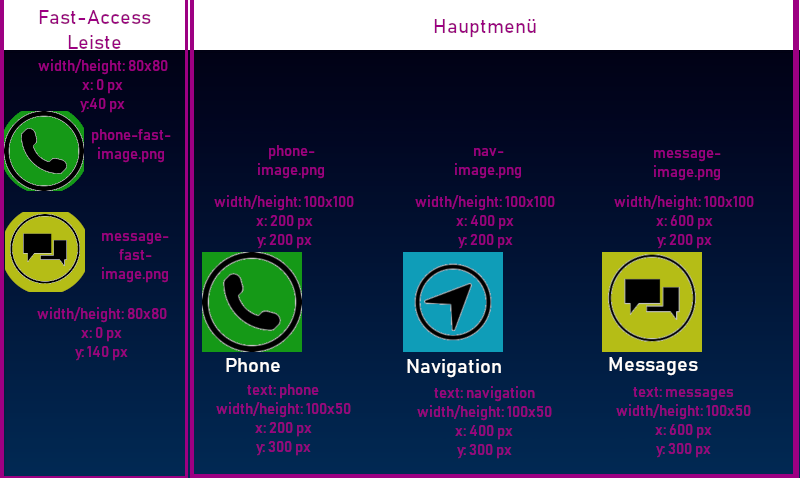
\includegraphics[width=\textwidth]{figures/Styleguide_Rahmen.png}
  \captionof{figure}{Styleguide}
  \label{fig:Styleguide}
\end{center}

Zusätzliche zu dieser grafischen Darstellung der Arbeitsaufgabe, wird noch eine textuelle Angabe erstellt, die zur Durchführung des Tests nötig ist.
Es werden insgesamt drei verschiedene Angaben erstellt, die in den Anhängen \ref{app:Aufgabe_Filter}, \ref{app:Aufgabe_Prototyp} und \ref{app:Aufgabe_Guide} zu finden sind.
Die ersten beiden dienen hierbei der Überprüfungen der Anpassungen.
Da ein Teil hiervon implementiert und der andere Teil mithilfe eines Prototypen umgesetzt wurde ist es hier nötig den Test in zwei Teile aufzuspalten, weshalb auch zwei getrennte Angaben existieren.
In Testaufgabe \ref{app:Aufgabe_Filter} galt es den implementierten Filter zu überprüfen, weshalb die Nutzer hier aufgefordert werden die drei Bilder für das Hauptmenü zu platzieren und mit Widget Feature Properties zu versehen.
Für diesen ersten Teil wird den Nutzern ein vorbereitetes Projekt mit den benötigten Assets zur Verfügung gestellt, um zu gewährleisten das alle mit einer identischen Ausgangssituation starten.
Es wird hier explizit nicht auf die implementierte Änderungen hingewiesen, da überprüft werden soll ob diese von den Nutzern intuitiv benutzt wird.
Um jedoch zu gewährleisten, dass jeder Nutzer das Filterfeld theoretisch nutzen könnte wird darum geben die Bilder mit Widget Feature Properties zu versehen.

Für Aufgabe \ref{app:Aufgabe_Prototyp} ist es notwendig den Übergang zu der Aufgabe innerhalb des Prototyp so nahtlos wie möglich zu gestalten und gleichzeitig wieder eine identische Ausgangssituation für alle Nutzer zu schaffen.
Das initiale Aussehen des Prototyp beinhaltet deshalb bereits die die drei bereits eingefügten Bilder im Hauptmenü, entspricht also der Situation mit der das vorherige Projekt in Guide von den Testpersonen verlassen wurde.
Da die Multiselektion eine Neuerung ist die eher unwahrscheinlich selbstständig von den Nutzern entdeckt wird, wird hier zu Anfang darauf hingewiesen das der vorliegende Prototyp Multiselektion unterstützt.
Mithilfe der Fast-Access Leiste, welche mithilfe von Templates modelliert werden soll, wird die Verlagerung der Funktion \glqq publish to template interface\grqq{} überprüft.
Ebenfalls wird in diesem Zug darauf hingewiesen, das nun auch die Bilder mithilfe von Multiselektion in Templates eingefügt werden können, jedoch ohne genaue Erklärung auf welche Art und Weise das funktioniert.
Abschließend sollen noch die Bilder und Labels positioniert und skaliert werden.
Es wird hier nocht noch einmal explizit auf die Multiselektion verwiesen, da herausgefunden werden soll inwiefern die Probanden dies nach der Information zu Anfang der Angabe intuitiv für die restliche Aufgabe nutzen.

Die letzte Aufgabe \ref{app:Aufgabe_Guide} dient zur Erlangung der Vergleichswerte für die Effizienz und wird deshalb in der unmodifizierten Version von Guide umgesetzt.
Da hier deshalb kein Übergang in den Prototyp notwendig ist ist eine zusammenhängende Arbeitsaufgabe ausreichend.
Die Probanden müssen hier die identische Aufgabe durchführen und werden, angepasst an die beiden vorherigen Angaben, in der Nutzung von Templates eingeschränkt oder dazu aufgefordert.
Den Nutzern hier ein komplett freies Arbeiten ist nicht möglich, da möglichst identische Arbeitsschritte getätigt werden müssen um einen validen Vergleich anstellen zu können.


\section {Ergebnisse}
Test fand mit 10 Testpersonen statt, Vergleich der Effizienz \cite{.h}

\paragraph{Ergebnisse altes Interface}
Filter: Bei 3 von 5 Probanden benutzt, Durchschnitt 2 Sekunden
Fehlerrate: 2 von 5 Nutzern ein Fehler

Publish: 3 von 5 Probanden gefunden, alle in 4,6 sek verlinkt
von 2 anderen nicht entdeckt, jedoch als Nützlich eingestuft
nachdem allen Hotspot erklärt wurde, Fehlerrate von 0

Multiselektion:
Bilder:
	Skalieren:
		Alle zusammen: 5 Nutzer in durch. 7,2 sek

	Positionieren:
		Mit Alignment: 1 Person in 5 sek
			Nutzungsfehler, sonst schneller
		Alle zusammen: 4 Personen in durch 3,5 sek
			identische Koordianten zusammen anpassen, danach einzelne Bilder wählen und anpassen
			Alignment entweder nicht gesehen oder als nicht relevant betrachtet

Texte:
	Skalieren:
		Alle zusammen: 4 Nutzer in durch. 8 sek

	Positionieren:
		Alignment an Bildern: Niemand
			Alignment ohnehin neu, kombi aus verschiedenen Elementen zu verwirrend
		
		Mit Alignment: 2 Personen in durch. 6 sek
			Erneut gleicher Fehler, deshalb längere Dauer
		Alle zusammen: 3 Personen in durch. 4,6 sek
			Gründe wie bei Bildern


Insert in Template: Niemand benutzt, wird als nicht intuitiv gewertet


\paragraph{Ergebnisse überarbeitetes Interface}
\paragraph{Vergleich}
